% Created 2017-11-11 Sat 20:34
\documentclass[11pt]{article}
\usepackage[utf8]{inputenc}
\usepackage[T1]{fontenc}
\usepackage{fixltx2e}
\usepackage{graphicx}
\usepackage{longtable}
\usepackage{float}
\usepackage{wrapfig}
\usepackage{rotating}
\usepackage[normalem]{ulem}
\usepackage{amsmath}
\usepackage{textcomp}
\usepackage{marvosym}
\usepackage{wasysym}
\usepackage{amssymb}
\usepackage{hyperref}
\tolerance=1000
\usepackage{minted}
\usepackage{fancyhdr}
\setcounter{secnumdepth}{-1} 
\pagestyle{fancy}
\fancyhead{} 
\rhead{\textit{Michael Laufer}}
\lhead{\textit{Numerical Methods Fall 2017, HW6}}
\small

\author{Michael Laufer}
\date{\today}
\title{HW2 Numerical Methods Fall 2017}
\hypersetup{
  pdfkeywords={},
  pdfsubject={},
  pdfcreator={Emacs 25.3.1 (Org mode 8.2.10)}}
\begin{document}

\maketitle
\section{Finite Difference - Poisson Equation}
\label{sec-1}
Given the Poisson equation:
\[
\frac{\partial^{2} \phi}{\partial x^{2}} + \frac{\partial^{2} \phi}{\partial y^{2}} = S_{\phi}
\]
Where $S_{\phi}$ is defined as:
\[
S_{\phi}=50000 \exp^{ -50 \left[ \left( 1 - x \right)^{2}  + y^{2} \right] } \cdot \left[ 100 \left( \left( 1-x^{2}  \right)  + y^{2} \right) -2 \right]
\]
Derichlet boundary conditions are given as functions defined on the square domain boundary. \\
The system has an analytical solution given by:
\[
\phi \left( x,y \right) = 500 e^{-50 \left[ \left(1-x \right)^{2} + y^{2}\right] } + 100x \left( 1-y \right)
\]
We will discretize the second order spatial derivatives with a 2nd order central differencing stencil which will lead to a 5 point stencil. The choice of using a central differencing stencil is appropriate as the Poisson equation is essentially an isotropic diffusion. In this fashion, the symmetric central differencing scheme matches the underlying physical phenomenon. 
\[
\frac{\partial^{2} \phi}{\partial x^{2}} = \frac{\phi_{i+1,j} + \phi_{i-1,j} -2\phi_{i,j} }{\left(\Delta x \right)^{2}}
\]

\[
\frac{\partial^{2} \phi}{\partial y^{2}} = \frac{\phi_{i,j+1} + \phi_{i,j-1} -2\phi_{i,j} }{\left(\Delta y \right)^{2}}
\]

\[
\frac{\partial^{2} \phi}{\partial x^{2}} + \frac{\partial^{2} \phi}{\partial y^{2}}  = \frac{\phi_{i+1,j} + \phi_{i-1,j} -2\phi_{i,j} }{\left(\Delta x \right)^{2}} + \frac{\phi_{i,j+1} + \phi_{i,j-1} -2\phi_{i,j} }{\left(\Delta y \right)^{2}} = S_{\phi} 
\]
This equation  shows the linear dependence of each node on its north, south, east, and west neighbors. 
This equation is then rearranged for each of the nodes into a full rank $nx$ X $ny$ matrix equation.

The following Numpy code snippet builds the coefficient matrix and RHS vector for the interior nodes. It follows Mazumder's derivation, but takes into account the slightly different Python array indexing: \\

\textbf{Numpy - Coef. Matrix, RHS Vector:} 
\begin{minted}[]{python}
A = np.zeros((nx*ny, nx*ny), dtype=float)     # Coef. Matrix
Q = np.zeros(nx*ny, dtype=float)              # RHS vector
dx = 1.0/(nx - 1)
dy = 1.0/(ny - 1)
dx2 = dx*dx
dy2 = dy*dy

for i in range(1, nx-1):
    for j in range(1, ny-1):
	k = (j-1)*nx + i -1                  # Running Index
	A[k,k] = -(2.0/dx2 + 2.0/dy2)
	A[k, k-1] = 1/dx2
	A[k, k+1] = 1/dx2
	A[k, k-nx] = 1/dy2
	A[k, k+nx] = 1/dy2
	Q[k] = S[j,i]
\end{minted}
The boundary nodes are dealt with in a similar manner. For example, for the left boundary of our domain:  \\

\textbf{Numpy - Left Boundary Example:} 
\begin{minted}[]{python}
i = 0                                      # Index for left boundary
for j in range(ny):
    k = (j-1)*nx + i -1
    A[k,k] = 1
    Q[k]  = phi_left[j]
\end{minted}

The corresponding matrix equation is solved using the built-in Numpy linear algebra solver. 
The system was solved for both $nx=ny=21$ and $nx=ny=41$, and the absolute error between the numerical solution and the analytical solution is plotted in the domain..

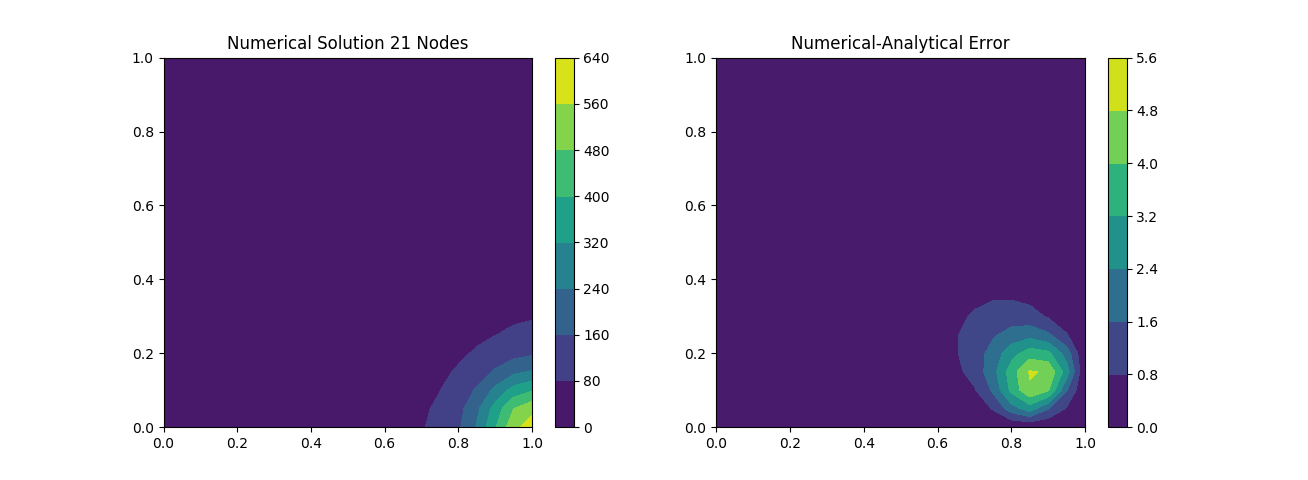
\includegraphics[width=15cm]{./figures/21node.png}


We can see that even with 21x21 nodes, a maximum error of less than 1\% compared to the anlaytical solution. 

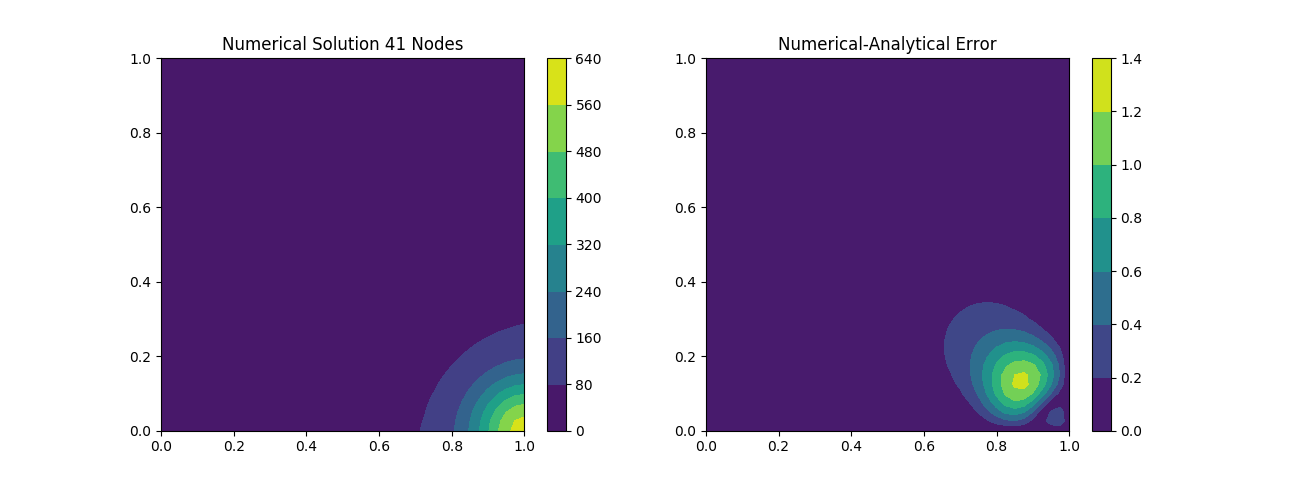
\includegraphics[width=15cm]{./figures/41node.png}


The 41x41 node solution shows a smoother contour plot, along with a substantially lower maximum error. We can see the same region with the maximal errors, which seems to correlate to the region of highest spatial gradients. The magnitude of the gradient in that region is clearly observed in the following surface plot solved with 101x101 nodes.

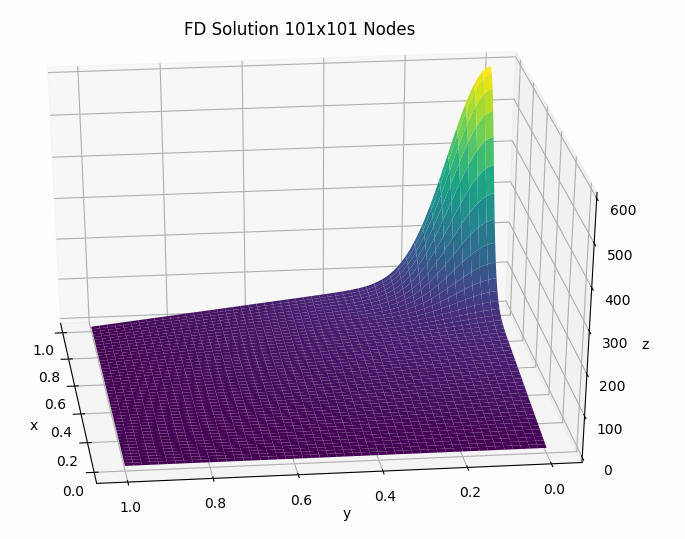
\includegraphics[width=15cm]{./figures/3d.png}

\newpage
\section{Appendix: Python Code}
\label{sec-2}
\begin{minted}[]{python}
import numpy as np
import matplotlib.pyplot as plt
from mpl_toolkits.mplot3d import Axes3D
from matplotlib import cm

nx = 21
ny = 21
x = np.linspace(0, 1, nx)
y = np.linspace(0, 1, ny)
xx, yy = np.meshgrid(x, y, sparse=True)

# Expressions
phi_analytical = 500*np.exp(-50*((1-xx)**2 + yy**2)) + 100*xx*(1-yy)
S = 50000*np.exp(-50*((1-xx)**2 + yy**2))*(100*((1-xx)**2 + yy**2) -2)
phi_right = 100*(1-y) + 500*np.exp(-50*(y**2))
phi_left = 500*np.exp(-50*(1+y**2))
phi_bottom = 100*(x) + 500*np.exp(-50*((1 - x)**2))
phi_top = 500*np.exp(-50*((1-x)**2 +1))

# Coef. Matrix, RHS Vector
A = np.zeros((nx*ny, nx*ny), dtype=float)
Q = np.zeros(nx*ny, dtype=float)
dx = 1.0/(nx - 1)
dy = 1.0/(ny - 1)
dx2 = dx*dx
dy2 = dy*dy

for i in range(1, nx-1):
    for j in range(1, ny-1):
	k = (j-1)*nx + i -1
	A[k,k] = -(2.0/dx2 + 2.0/dy2)
	A[k, k-1] = 1/dx2
	A[k, k+1] = 1/dx2
	A[k, k-nx] = 1/dy2
	A[k, k+nx] = 1/dy2
	Q[k] = S[j,i]

# Left Boundary
i = 0
for j in range(ny):
    k = (j-1)*nx + i -1
    A[k,k] = 1
    Q[k]  = phi_left[j]

# Right Boundary
i = nx - 1
for j in range(ny):
    k = (j-1)*nx + i -1
    A[k,k] = 1
    Q[k]  = phi_right[j]

# Bottom Boundary
j = 0
for i in range(nx):
    k = (j-1)*nx + i -1
    A[k,k] = 1
    Q[k]  = phi_bottom[i]

# Top Boundary
j = ny - 1
for i in range(nx):
    k = (j-1)*nx + i -1
    A[k,k] = 1
    Q[k]  = phi_top[i]

# Solve and unpack solution
phi2d = np.zeros((nx,ny))
phi1d = np.linalg.solve(A,Q)    
for i in range(nx):
    for j in range(ny):
	k = (j-1)*nx + i - 1
	phi2d[j,i] = phi1d[k]

# Absolute error
error = np.abs(phi2d - phi_analytical)

# 2D plot
plt.figure(1)
plt.subplot(121)
plt.contourf(x,y,phi2d)
plt.colorbar()
plt.title('Numerical Solution 21 Nodes')
plt.subplot(122)
plt.contourf(x,y,error)
plt.colorbar()
plt.title('Numerical-Analytical Error')
plt.title('Absolute Error')


# 3d plot
fig = plt.figure(figsize=(11, 7), dpi=100)
ax = fig.gca(projection='3d')
ax.plot_surface(xx, yy, phi2d, cmap=cm.viridis, rstride=2, cstride=2)
ax.set_xlabel('x')
ax.set_ylabel('y')
ax.set_zlabel('z')
plt.title('FD Solution 3D')

plt.show()
\end{minted}
% Emacs 25.3.1 (Org mode 8.2.10)
\end{document}